%!TEX root=../thesis.tex
\chapter{Experiments} \label{cha:experiments}

This chapter outlines in detail all the experiments run on the test application.
Moreover, it provides also a discussion about the outcomes of the analysis. 


\section{First measurements}
The first measurements are obtained using the Web Tracing Framework presented in
Section \ref{sec:wtf} and following the metodologies depicted in Sections
\ref{sec:assumptions} and \ref{sec:procedure}.

The very first approach for profiling the navigator can be considered as an
exploratory phase. All the default events available to the framework are
used, resulting in a considerable amount of data. Fortunately the WTF interface
displays the trace in a very neat way, allowing the user to easily navigate
through the time series of the function calls. Moreover, based on this step,
a selection of the interesting function calls is outlined in order to narrow the
search field. The resulting list of WebGL primitives\footnote{A detailed description
of the WebGL APIs can be found at the following link:
\url{https://developer.mozilla.org/it/docs/Web/API/WebGL_API}.} is presented in
Table \ref{tab:webgl_function_list}
\begin{table}[!htb]
    \centering
    \caption{The list of the WebGL function of interest.}
    \label{tab:webgl_function_list}
    \begin{tabular}{|lllll|}
        \hline
        bindBuffer    & viewport        & clearColor    & bindTexture & uniformMatrix4v \\
        bufferSubData & clear           & createTexture & pixelStorei & linkProgram     \\
        disable       & bindFrameBuffer & activeTexture & textImage2D & \\
        \hline                
    \end{tabular}
\end{table}

After some trial-and-error tests, the trace extracted from the ``no-map'' scenario
is chosen as the first to be analyzed more in detail. Figure \ref{img:no_map_overview}
depicts a graphical representation of the trace, where every colored vertical bar
symbolizes an occurrence of the event/function call tracked by the tool. As it
is possible to notice, all of them are arranged into fairly regular groups.
\begin{figure}[!htb]
    \center{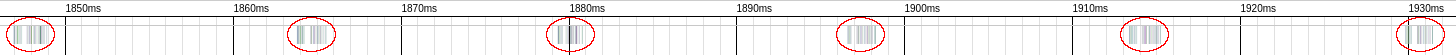
\includegraphics[width=1\linewidth]{no_map_overview.png}}
    \caption{An example trace highlighting the function groups.}
    \label{img:no_map_overview}
\end{figure}

Furthermore, every group starts with a \emph{bindBuffer} call; this function is
responsible for binding a buffer object containing vertexes and/or colors to the
current WebGL context. Essentially it marks an arbitrary buffer to be the current
one where all the other WebGL functions work on. This is necessary due to the
ability of the GPU process to deal with only one data structure at a time. Hence,
it is possible to virtually split the trace into small groups by means of the
\emph{bindBuffer} function.\\
After identifying the recurrent structure of the trace, it is possible to check
which are the recurrent WebGL functions in each group and to gather them into
macro-operations sets. After checking what is the specific task of every
function, it became clear that they belong to three different scopes:
\begin{itemize}
    \item \emph{initialization/load data}: every WebGL function in this group
        is responsible for preparing the data structures to be loaded in memory
        and for copying all the needed data.
    \item \emph{modify data}: these functions actually work on the vertex/color
        buffer to modify the data, especially via matrix operations.
    \item \emph{display/draw}: this group is the one that sends the commands
        that are actually used by the GPU to draw the shapes on the screen.
\end{itemize}

A more detailed functions-to-groups mapping is shown in Table
\ref{tab:webgl_func_mapping}.

\begin{table}[!htb]
    \centering
    \caption{WebGL functions-to-groups mapping.}
    \label{tab:webgl_func_mapping}
    \begin{tabular}{|l|l|l|}
        \hline
        \textbf{Initialization/load data} & \textbf{Modify data} & \textbf{Display/draw} \\ \hline
        bindBuffer/bindFramebuffer & uniformMatrix3fv/uniformMatrix4fv & drawElements \\
        enable/disable & uniform[1\(\vert\)2\(\vert\)3\(\vert\)4][f\(\vert\)i\(\vert\)iv\(\vert\)fv] & drawArray \\
        viewport & bindTexture/activeTexture &  \\
        clear/clearColor & bufferSubData &  \\
        cullFace &  &  \\
        depthCompare &  &  \\
        useProgram &  &  \\
        colorMask &  &  \\
        \hline
    \end{tabular}
\end{table}

Another important aspect to be noticed is how the timings fluctuate during the
application run. As it is possible to see from Figure \ref{img:no_map_example},
there can be outliers where the response time of the application is significantly
smaller or larger with respect to all the rest of the trace.
\begin{figure}[!htb]
    \center{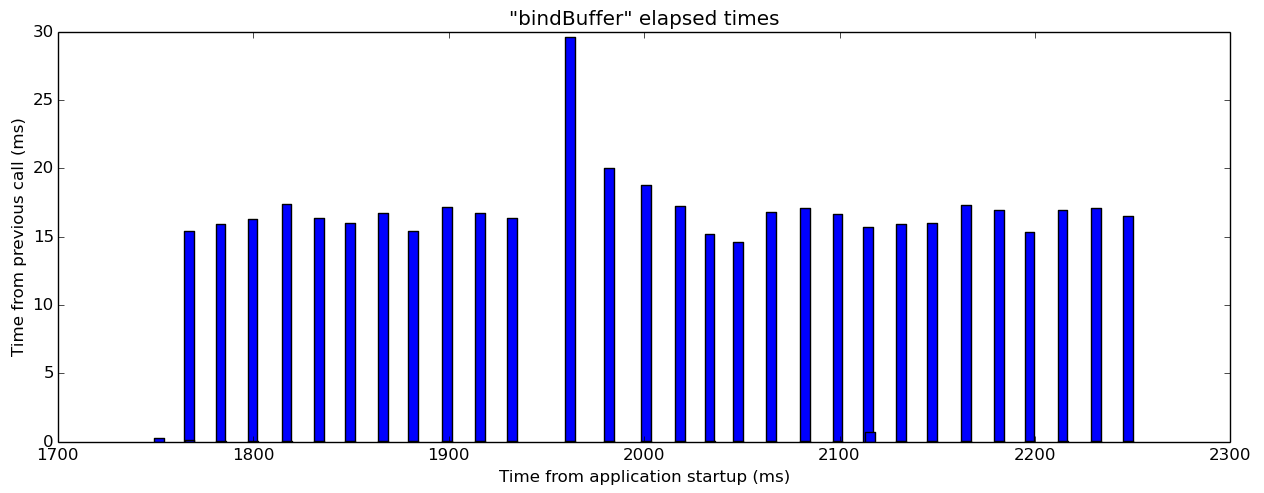
\includegraphics[width=0.75\linewidth]{500ms_1_no_map.png}}
    \caption{Another trace extracted from the ``no-map'' scenario.}
    \label{img:no_map_example}
\end{figure}
This fluctuating trend can have several justifications. Since the WTF is able to
measure only the response times of the test application with a precision of
\(\pm 0.5\,ms\), the bar chart shown
in Figure \ref{img:no_map_example} is displaying on the Y axes a value which can
be computed as follows:
\begin{equation*}
    response\_time = computation\_time + interference
\end{equation*}

The \emph{interference} component in the formula just above is clearly due to the
big OS stack which lies between the application JavaScript code runnint inside the
browser and the Mesa 3D graphics driver, which is part of the Linux OS kernel.
Thus, this issue has to be reduced to the minimum in order not to jeopardize the
validity of all the results presented in this chapter. One possibility to mitigate
the interference from higher priority tasks is to assign higher or real-time priorities
to the entire Googhe Chrome instance using the \emph{nice}~\cite{aas2005understanding}
tool. Another approach includes directly changing the scheduling policy via the
\emph{chrt}\footnote{\url{http://man7.org/linux/man-pages/man1/chrt.1.html}.}
utility to use different scheduling algorithms. It is possible to state that no
noteworthy difference can be seen in the response times after applying the
methods proposed above. For this reason, the \emph{computation\_time} component
can be considered as the unique responsible for the timings fluctuations.

Moreover, after dividing all the WebGL functions into macro-operations groups
(see Table \ref{tab:webgl_func_mapping}). As it is possible to see from Figure
\ref{img:no_map_groups}, this ``grouped'' bar chart is very useful to understand
the weight of every set of operations with respect to the time elapsed between
each \emph{bindBuffer} function call.
\begin{figure}[!htb]
    \center{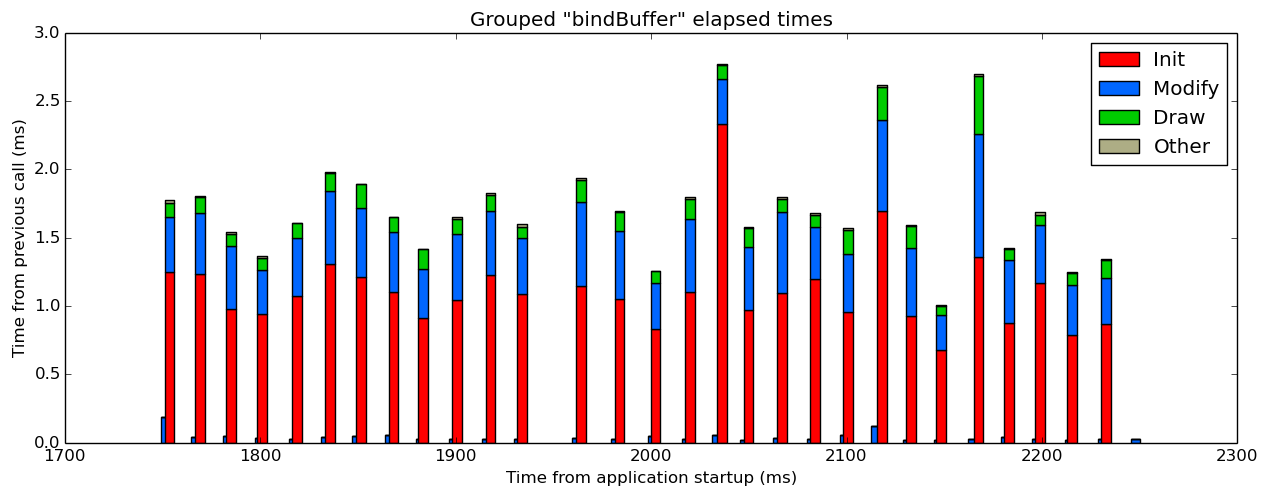
\includegraphics[width=0.8\linewidth]{500ms_1_no_map_groups.png}}
    \caption{An example of a grouped bar chart computed from a trace.}
    \label{img:no_map_groups}
\end{figure}

A comparison between extensive 2D and 3D tests showed that response times
during 3D rendering are slightly higher and more prone to fluctuations. This is
certainly due to the different computation workloads which can significantly change
over time, depending on the complexity of the scene to be rendered.

Finally, this analysis work allows to discover a preliminary task model where
each job of the rendering task can be divided into three logically different
parts. A graphical rappresentation is given in Figure \ref{img:call_arrival}.

\begin{figure}[!htb]
    \center{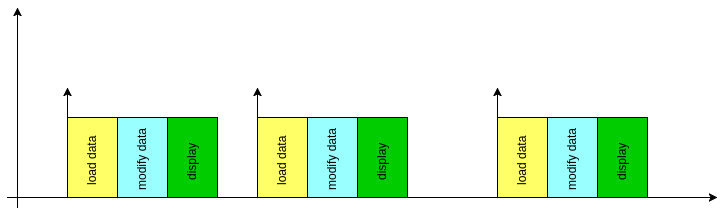
\includegraphics[width=0.6\linewidth]{call_arrival.png}}
    \caption{The function calls arrival approximate model with the different groups.}
    \label{img:call_arrival}
\end{figure}


\section{A fine-grained model}

